\chapter{State of Research}
\label{chap:state-of-research}

This chapter provides the background and research basis needed for the development of the diagnostic method. This literature review is a continuation of the work carried out by Kouom Nankam with additional studies that are especially relevant to the focus of this thesis \cite{Kouom2026}. It first introduces the basic medical principles of malaria diagnosis and the main concepts of deep learning that are relevant for this work. Based on this, existing AI-based approaches for malaria diagnosis are reviewed and compared with regard to their data, model types, evaluation methods, and the actual practical use. This chapter starts with the basic medical background of malaria diagnosis and then introduces the deep learning methods that are relevant for this work. After that, previous research approaches are presented and compared. The chapter ends by identifying the main research gap and explaining how it is related to this thesis.

\section{Literature Basis and Previous Work}
\label{sec:literature_basis}

The literature review in this thesis is based on previous work carried out at HAWK Göttingen. In February 2026, Kouom Nankam completed a systematic literature review on AI-based malaria diagnosis using microscopic blood images. His research covered publications from 2022 to 2025 from IEEE Xplore, ScienceDirect, SpringerLink, and PubMed. His search used combinations of terms such as ''malaria diagnosis'', ''deep learning'', ''convolutional neural networks'', ''vision transformer'', and ''microscopic blood smear''. His analysis first began with reviewing the titles and abstracts to check their relevance. After that, the selected studies were read and analysed in full \cite{Kouom2026}.

The review contained 38 references and focused on datasets, preprocessing methods, model architectures, training and validation strategies, evaluation metrics, explainability, and practical applicability. The work was literature-based and did not include its own model implementation or experimental evaluation \cite{Kouom2026}.

Although the review covered different AI approaches for malaria diagnosis, it focused mainly on thin blood smear images. Kouom explicitly excluded thick blood smear analysis from the scope of the work. He pointed out that thick blood smears provide higher sensitivity for parasite detection, but that their complex visual structure and high cell density make automated image analysis and reliable annotation more difficult \cite{Kouom2026}. This limitation is relevant for the present thesis since the diagnostic method developed here focuses specifically on thick blood smear images.

To extend the previous literature review, an additional search was carried out for studies that were directly relevant to the research questions of this thesis. Search terms included combinations of ''malaria'', ''thick blood smear'', ''deep learning'', ''MobileNet'', ''object detection'', ''image resolution'', ''smartphone microscopy'', and ''explainable AI''. The identified studies were reviewed with focus on the parts relevant to this thesis, especially the methods, tools, datasets, and reported results. The findings were then compared with the previous HAWK literature review to avoid unnecessary duplication. Particular attention was given to studies involving thick blood smear images, patient-wise evaluation, reduced image resolution, and explainability.

\begin{table}[htbp]
    \centering
    \caption{Comparison of the HAWK literature review and the literature review of this thesis.}
    \label{tab:literature_review_comparison}
    \begin{tabularx}{\textwidth}{|p{3.2cm}|X|X|}
        \hline
        \textbf{Aspect} & \textbf{Kouom Nankam} & \textbf{This thesis} \\
        \hline
        Literature scope & Publications from 2022--2025 & Previous review extended with additional relevant studies \\
        \hline
        Blood smear type & Mainly thin blood smears. Thick-smear analysis excluded from the review scope & Mainly thick blood smears, thin blood smears included only in the literature review \\
        \hline
        Main focus & General state of AI-based malaria diagnosis & AI-based diagnosis with focus on classification, image resolution, efficiency, and explainability \\
        \hline
        Studies used & 38 references & 35 references including the work of Kouom Nankam\\
        \hline
        Experimental work & No implementation or experiments & Model implementation, training, testing, and benchmarking \\
        \hline
    \end{tabularx}
\end{table}

\FloatBarrier



\section{Malaria and Microscopic Diagnosis}
\label{sec:malaria_microscopy}

Malaria is an infectious disease caused by parasites from the genus Plasmodium. Five species are known to cause malaria in humans: P. falciparum, P. vivax, P. ovale, P. malariae, and P. knowlesi. Among them, P. falciparum is the most dangerous species and is responsible for most deaths caused by severe malaria \cite{Maturana2022}. During the blood stage of the infection, different parasite stages can be seen under the microscope. These include immature trophozoites, also known as ring forms, mature trophozoites, schizonts, and gametocytes \cite{Maturana2022}. These different stages are important for the microscopic diagnosis of malaria.

Giemsa staining is commonly used to make malaria parasites visible in blood smears. The WHO recommends Giemsa staining for both thick and thin blood films \cite{WHO2016Giemsa}. Before staining, the thin blood film is fixed with methanol. The thick blood film should not come into contact with methanol because the red blood cells need to undergo haemolysis. After staining, the slides are rinsed with buffered water and left to dry before they are examined under the microscope \cite{WHO2016Giemsa}.

Two main types of blood smears are used for microscopic malaria diagnosis: thick and thin blood smears. Thick smears are mainly used to check whether malaria parasites are present, while thin smears preserve the structure of the red blood cells and are therefore more suitable for identifying the Plasmodium species \cite{Maturana2022}.

Figure~\ref{fig:thick_thin_smear} shows the visual difference between a thick and a thin Giemsa-stained blood smear.

\begin{figure}[htbp]
    \centering
    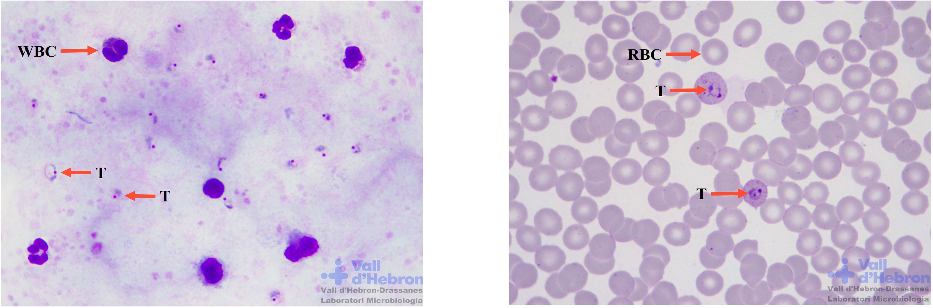
\includegraphics[width=0.8\textwidth]{thin-vs-thick.pdf}
    \caption{Comparison of Giemsa-stained blood smears. The left image shows a thick blood smear and the right image shows a thin blood smear. Source:  Maturana et al. \cite{Maturana2022}.}
    \label{fig:thick_thin_smear}
    \vspace{-0.3cm}
    \end{figure}

\FloatBarrier

In the figure, WBC stands for white blood cells, RBC for red blood cells, and T for trophozoites.

Thick blood smears are more sensitive than thin blood smears and can therefore detect lower parasite levels. Maturana et al. report that thick blood smears are approximately 20 to 40 times more sensitive than thin blood smears \cite{Maturana2022}.

Thin blood smears, on the other hand, keep the individual red blood cells visible. This makes it possible to examine the parasites together with the infected cells and makes species identification easier. The main differences between thick and thin blood smears are shown in Table~\ref{tab:thick_thin_comparison} \cite{Maturana2022}.

\begin{table}[htbp]
    \centering
    \caption{Comparison of thick and thin blood smears for malaria microscopy.}
    \label{tab:thick_thin_comparison}
    \begin{tabularx}{\textwidth}{|p{3.2cm}|X|X|}
        \hline
        \textbf{Aspect} & \textbf{Thick blood smear} & \textbf{Thin blood smear} \\
        \hline
        Main purpose &
        Detection and screening of malaria parasites &
        Identification of the Plasmodium species \\
        \hline
        Sensitivity &
        Higher, reported to be about 20--40 times more sensitive &
        Lower compared with thick smears \\
        \hline
        Red blood cells &
        Broken down during staining &
        Remain intact \\
        \hline
        Parasite visibility &
        Parasites are concentrated in a dense smear area &
        Parasites can be examined inside individual red blood cells \\
        \hline
        Image structure &
        Dense and less clearly structured &
        Individual cells can be seen more clearly \\
        \hline
    \end{tabularx}
\end{table}

\FloatBarrier

Thick blood smears can also be used to estimate the parasite density, not only to detect an infection. For this, the number of parasites is counted together with the number of white blood cells (WBCs). According to the WHO procedure, these values can then be used to calculate the parasite density \cite{WHO2016ParasiteCounting}:

\begin{equation}
D =
\frac{N_P \cdot C_{\mathrm{WBC}}}
     {N_{\mathrm{WBC}}},
\label{eq:parasite_density}
\end{equation}
where $D$ is the estimated parasite density in parasites/$\mu$L, $N_P$ is the number of parasites counted, $N_{\mathrm{WBC}}$ is the number of white blood cells counted, and $C_{\mathrm{WBC}}$ is the patient's white blood cell concentration per $\mu$L.

If the actual WBC concentration is not available, the WHO recommends using an assumed value of 8000 WBC/$\mu$L \cite{WHO2016ParasiteCounting}. Equation~\ref{eq:parasite_density} then becomes

\begin{equation}
D =
\frac{N_P \cdot 8000}
     {N_{\mathrm{WBC}}}.
\label{eq:parasite_density_who}
\end{equation}

Parasite density estimation is not part of the method developed in this thesis. The equations are only included to show how parasite concentration is calculated during conventional microscopic examination. The task of this work focuses instead on classifying thick blood smear images as infected or uninfected.

Although thick blood smears are very sensitive for parasite detection, their image structure makes automatic analysis more difficult. In contrast to thin smears, individual red blood cells are no longer clearly visible, and parasites appear together with other stained blood components and possible artefacts \cite{Yang2020}. Kouom Nankam also describes the complex structure and high cell density of thick smears as challenges for automated image analysis and annotation \cite{Kouom2026}. For this reason, this thesis focuses specifically on the automatic classification of thick blood smear images. Later experiments also investigate how reduced image resolution affects this task.

\section{Deep Learning Fundamentals}
\label{sec:deep_learning_fundamentals}

Since this thesis is based on deep learning, this section introduces the main concepts that are relevant for the developed method. It first explains the basic idea of deep learning and then focuses on convolutional neural networks, transfer learning, image analysis tasks, and the evaluation metrics used later in this work.

\subsection{Convolutional Neural Networks}

{\color{blue}  
A CNN processes an image through several layers. The first layers usually learn simple image features such as edges, colours, and textures. Deeper layers combine these simple features into more complex patterns that are useful for the final prediction \cite{Goodfellow-et-al-2016}. This hierarchical feature extraction is one of the main reasons why CNNs are suitable for image classification.

The main operation of a CNN is the convolution. A small filter, also called a kernel, moves across the input image or feature map and calculates a new feature map. Following the standard formulation of convolution used in deep learning \cite{Goodfellow-et-al-2016}, A simplified two-dimensional convolution operation used in CNNs can be written as:

\begin{equation}
Y(i,j) =
\sum_{m}\sum_{n}
X(i+m,j+n)K(m,n) + b
\label{eq:convolution}
\end{equation}

where $X$ represents the input, $K$ is the convolution kernel, $b$ is a bias term, and $Y$ is the resulting feature map. During training, the values of the kernels are learned automatically from the data.


After a convolution, an activation function is normally applied. A commonly used activation function is the Rectified Linear Unit (ReLU) \cite{Goodfellow-et-al-2016}, which is defined as:

\begin{equation}
\mathrm{ReLU}(x) = \max(0,x)
\label{eq:relu}
\end{equation}


ReLU keeps positive values while setting negative values to zero. This introduces non-linearity and allows the network to learn more complex relationships between the input image and the target class \cite{Goodfellow-et-al-2016}.
}

\begin{tcolorbox}[
    colback=gray!15,
    colframe=gray!50,
    boxrule=0.5pt
]

\textbf{Type and extent of AI use}

Claude was used to extract useful information from the book by Goodfellow et al. The extracted information were used for the deep learning fundamentals section.

\vspace{0.4cm}

\textbf{The individual contribution}

The extracted information were selected based on what was needed for this section and was used according to the structure of the section. The information was then used to explain the main deep learning fundamentals that are relevant to this thesis.

\vspace{0.4cm}

\textbf{Critical evaluation of the AI contribution}

The book by Goodfellow et al. contains more than 800 pages. By using Claude, the relevant information could be found and extracted more efficiently. This also saved time that could be used to analyse other references that are more directly related to the topic of this thesis.

\end{tcolorbox}

The development of CNN architectures has resulted in networks with different levels of complexity. AlexNet demonstrated the potential of deep CNNs for large-scale image classification \cite{Krizhevsky2012}. VGG later increased the network depth using repeated small convolution filters \cite{Simonyan2015}. ResNet introduced residual connections that allow information to bypass individual layers and make the training of deeper networks easier \cite{He2016}. Other architectures focus more strongly on computational efficiency. MobileNet uses depthwise separable convolutions to reduce computational cost \cite{Howard2017}, while SqueezeNet was designed to strongly reduce the number of model parameters \cite{Iandola2016}. These differences between CNN architectures are relevant when selecting a model based not only on classification performance but also on computational requirements.

CNNs are not the only approach used in modern image analysis. Vision Transformers (ViTs) apply the Transformer concept to images by dividing an image into smaller patches and processing the relationships between these patches using attention mechanisms \cite{Dosovitskiy2021}. 

\subsection{Transfer Learning}


Training a deep neural network completely from scratch generally requires a large amount of labelled data. Transfer learning provides an alternative by reusing knowledge learned from another task. In transfer learning, knowledge from a previously learned task is transferred to support learning on a new task \cite{PanYang2010}.

For image classification, pretrained models can be used as a starting point for a new task. The learned features of these models can then be reused for another image classification problem \cite{Rajaraman2018}.

When pretrained models are further trained using a new dataset, this process is commonly referred to as fine-tuning. This approach is also used in malaria image analysis, for example by Maturana et al., who fine-tuned pretrained detection models using their thick blood smear dataset \cite{Maturana2023}.

{\color{blue}  
During training, the model parameters are updated by minimising a loss function. For classification tasks, cross-entropy loss is commonly used to measure the difference between the predicted class probabilities and the true class label \cite{Goodfellow-et-al-2016}. For a classification problem with \(C\) classes, the cross-entropy loss can be written as:

\begin{equation}
L = -\sum_{c=1}^{C} y_c \log(p_c)
\label{eq:cross_entropy}
\end{equation}

where \(y_c\) represents the true class label and \(p_c\) the predicted probability for class \(c\).

During model development, the available data are normally separated into training, validation, and test data. The training set is used to update the model parameters. The validation set is used to observe the model during development and to support decisions such as model or hyperparameter selection. The test set should remain separate and is used for the final evaluation of the trained model. This separation is important because evaluating the model on data that were already used during training can lead to an unrealistic estimation of its performance \cite{Goodfellow-et-al-2016}.
}

\begin{tcolorbox}[
    colback=gray!15,
    colframe=gray!50,
    boxrule=0.5pt
]

\textbf{Type and extent of AI use}

Claude was used to extract useful information from the book by Goodfellow et al. The extracted information was used for the deep learning fundamentals section.

\vspace{0.4cm}

\textbf{The individual contribution}

The extracted information was selected based on what was needed for this section and was arranged according to the structure of the chapter. It was then used to explain the main deep learning fundamentals that are relevant to this thesis.

\vspace{0.4cm}

\textbf{Critical evaluation of the AI contribution}

The book by Goodfellow et al. contains more than 800 pages. By using Claude, the relevant information could be found and extracted more efficiently. This also saved time that could be used to analyse other references that are more directly related to the topic of this thesis.

\end{tcolorbox}

\subsection{Image Analysis Tasks}

The studies reviewed in this thesis use different image analysis tasks. The main tasks relevant to this work are classification, object detection, and segmentation.

Image classification assigns a class to an image or image region. For example, a binary classifier can distinguish between infected and uninfected samples \cite{Rajaraman2018}. However, classification does not show where an object is located in the image.

Object detection also identifies the position of objects, usually using bounding boxes. YOLO is a common example of an object detection approach \cite{Redmon2016}. In malaria analysis, this can be used to locate individual parasites or blood cells.

Image segmentation works at pixel level and assigns a label to individual pixels \cite{Kassim2021RBCNet}. This allows structures such as cells or background regions to be separated more precisely.

Since these tasks solve different problems, their results and evaluation metrics should not be compared directly without considering the task being performed.

\subsection{Evaluation Metrics}

The performance of a binary classification model can be described using true positives ($TP$), true negatives ($TN$), false positives ($FP$), and false negatives ($FN$). In this thesis, infected samples are treated as the positive class and uninfected samples as the negative class. The following evaluation metrics are based on these values \cite{Delahunt2024}:

\begin{equation}
\mathrm{Accuracy} =
\frac{TP+TN}
{TP+TN+FP+FN}.
\label{eq:accuracy}
\end{equation}

Sensitivity, also called recall, describes how many infected samples are correctly identified:

\begin{equation}
\mathrm{Sensitivity} =
\mathrm{Recall} =
\frac{TP}
{TP+FN}.
\label{eq:sensitivity}
\end{equation}

Specificity describes how many uninfected samples are correctly identified:

\begin{equation}
\mathrm{Specificity} =
\frac{TN}
{TN+FP}.
\label{eq:specificity}
\end{equation}

Precision describes how many samples predicted as infected are actually infected:

\begin{equation}
\mathrm{Precision} =
\frac{TP}
{TP+FP}.
\label{eq:precision}
\end{equation}

The F1-score combines precision and recall:

\begin{equation}
F_1 =
2 \cdot
\frac{\mathrm{Precision}\cdot\mathrm{Recall}}
{\mathrm{Precision}+\mathrm{Recall}}.
\label{eq:f1_score}
\end{equation}

These metrics describe different parts of the model performance. Sensitivity is especially important for showing how reliably infected samples are detected, while specificity shows how reliably uninfected samples are identified \cite{Delahunt2024}.

The Receiver Operating Characteristic (ROC) curve shows the relationship between the true-positive rate and false-positive rate at different classification thresholds. The Area Under the ROC Curve (ROC-AUC) summarises this behaviour in one value. Delahunt et al. point out that metrics such as ROC-AUC and F1 should be interpreted carefully in malaria diagnosis and emphasise the importance of patient-level evaluation \cite{Delahunt2024}.

Object detection studies can also report Average Precision (AP) or mean Average Precision (mAP). These metrics are relevant to the object detection studies discussed later in this chapter, but they are not used to evaluate the classifiers developed in this thesis.

\section{AI-Based Malaria Diagnosis from Microscopic Images}
\label{sec:ai_malaria_diagnosis}

Automated malaria diagnosis has developed from traditional image-processing methods towards deep learning-based approaches. Earlier methods often used manually designed image features, while more recent approaches use convolutional neural networks to learn relevant features directly from microscopic images \cite{Maturana2022,Quinn2016}.

The literature includes different tasks such as image classification, parasite detection, species identification, and patient-level diagnosis. Kassim et al., for example, combined parasite detection and classification to distinguish between P. falciparum, P. vivax, and uninfected samples at image and patient level \cite{Kassim2021}.

Both thin and thick blood smear images have been used for automated malaria analysis. Thick blood smears are especially relevant for parasite screening, but their dense image structure makes automatic analysis more difficult \cite{Maturana2022}. For this reason, the following sections focus mainly on approaches using thick blood smear images.

Smartphone-based microscopy has also become relevant for automated malaria diagnosis. Quinn et al. used CNNs for malaria detection from thick blood smear images captured using smartphones \cite{Quinn2016}. Such approaches are relevant to this thesis because the future system is also intended to combine a microscope, smartphone, and automated image analysis.

\section{Thick Blood Smear Datasets and Image Acquisition}
\label{sec:datasets_acquisition}

For the practical work of this thesis, three thick blood smear datasets were considered: the datasets provided by the National Library of Medicine (NLM), the Uganda dataset presented by Quinn et al., and the Drassanes--Vall d'Hebron dataset.

The NLM provides thick blood smear images from patients infected with P. falciparum and P. vivax, as well as images from uninfected patients. Yang et al. published a dataset containing 1819 images from 150 patients infected with P. falciparum. The images were captured using a smartphone camera connected to a microscope and contain 84 961 manually annotated parasites \cite{Yang2020}. Kassim et al. later used a combined NLM collection containing 5972 images from 350 patients with P. falciparum, P. vivax, and uninfected samples \cite{Kassim2021}.

The Uganda dataset presented by Quinn et al. contains 1182 thick blood smear images with 7245 annotated parasites \cite{Quinn2016}. The images were captured using a smartphone microscope setup. Since the dataset contains malaria-positive images and parasite-level annotations, it is mainly suitable for parasite detection rather than infected-versus-uninfected classification. In this thesis, it was later used as an external test dataset.

The Drassanes--Vall d'Hebron dataset contains 2571 labelled thick blood smear images \cite{VallHebron2025}. The images were captured using either a Leica microscope camera or a Samsung Galaxy S20 connected to the microscope. The dataset contains different Plasmodium species and object-level annotations. However, all included thick blood smear samples are malaria-positive, which means that the dataset cannot directly provide an uninfected class for the binary classification task used in this thesis.

Table~\ref{tab:malaria_datasets} gives an overview of the three datasets.

\begin{table}[htbp]
    \centering
    \caption{Overview of the thick blood smear datasets considered in this thesis.}
    \label{tab:malaria_datasets}
    \begin{tabularx}{\textwidth}{|p{2.7cm}|X|X|X|}
        \hline
        \textbf{Dataset} &
        \textbf{Size} &
        \textbf{Acquisition} &
        \textbf{Main characteristics} \\
        \hline

        NLM datasets &
        5972 images / 350 patients reported by Kassim et al. &
        Smartphone microscopy &
        P. falciparum, P. vivax, and uninfected samples \cite{Yang2020,Kassim2021} \\
        \hline

        Uganda / AIR &
        1182 images / 7245 annotated parasites &
        Smartphone-microscope setup &
        Malaria-positive thick smear images with parasite-level annotations \cite{Quinn2016} \\
        \hline

        Drassanes--Vall d'Hebron &
        2571 labelled images &
        Leica microscope camera or Samsung Galaxy S20 &
        Multiple Plasmodium species and object-level annotations; malaria-positive samples \cite{VallHebron2025} \\
        \hline

    \end{tabularx}
\end{table}

\FloatBarrier

The NLM datasets were selected for the main training and internal evaluation because they contain both infected and uninfected patients. The P. falciparum and P. vivax images could therefore be combined into one infected class and compared with the uninfected class.

The high original image resolution was also useful for the resolution experiments in this thesis because lower-resolution versions could be generated from the same images. The final dataset preparation, class definition, patient-wise splitting, and preprocessing are described in Chapter~\ref{chap:implementation}.

\section{CNN-Based Classification Approaches}
\label{sec:cnn_classification}

CNNs are widely used for automated malaria image classification because they can learn relevant image features directly from the training data. Different approaches have used pretrained CNNs, custom CNN architectures, or a combination of detection and classification.

Rajaraman et al. investigated pretrained CNNs for the classification of parasitized and uninfected cells in thin blood smear images \cite{Rajaraman2018}. The evaluated architectures included AlexNet, VGG-16, ResNet-50, Xception, and DenseNet-121. The study showed that features learned by pretrained CNNs can be reused for malaria image classification.

For thick blood smears, Yang et al. developed a method that combines Iterative Global Minimum Screening (IGMS) with a custom CNN \cite{Yang2020}. IGMS first selects possible parasite candidates from the microscopic image. The CNN then classifies the extracted patches as parasite or background. Their CNN achieved an accuracy of 93.46\%, a sensitivity of 92.59\%, and a specificity of 94.33\%. The study is particularly relevant because it uses smartphone-acquired thick blood smear images. However, the classification is performed on selected image patches instead of the complete microscopic image.

Kassim et al. also combined detection and classification for thick blood smear images \cite{Kassim2021}. Their PlasmodiumVF-Net first detects parasite candidates using Mask R-CNN and then uses ResNet50 to reduce false-positive detections. The final system provides decisions at image and patient level and distinguishes between P. falciparum, P. vivax, and uninfected samples. This study is especially relevant because it uses the same NLM dataset family that is used in this thesis.

These studies show that CNNs can be used in different ways for malaria analysis. Rajaraman et al. used pretrained CNNs for cell classification, while Yang et al. and Kassim et al. combined candidate detection with CNN-based classification. In contrast, this thesis investigates direct binary classification of complete thick blood smear images without a separate parasite detection step.

ResNet50 and ResNet18 are used as the main residual architectures in this thesis. Lightweight architectures such as MobileNet are discussed separately in Section~\ref{sec:lightweight_networks}.

\section{Object Detection Approaches}
\label{sec:object_detection}

Object detection is used when individual parasites or blood cells need to be located inside a microscopic image. Unlike image classification, the model does not only predict a class but also identifies the position of the detected objects. This is mostly useful in malaria analysis because several parasites can appear within the same microscopic field.

Maturana et al. investigated object detection on thick blood smear images as part of the iMAGING system \cite{Maturana2023}. They compared YOLOv5x, Faster R-CNN, SSD, and RetinaNet using a dataset of 2571 labelled images. The models detected leukocytes, early trophozoites, and mature trophozoites. YOLOv5x achieved a precision of 92.10\%, a recall of 93.50\%, an F-score of 92.79\%, and an mAP@0.5 of 94.40\%. This study is particularly relevant because it combines thick blood smear analysis with smartphone-based image acquisition and automated microscopy.

Vásquez Ascate et al. developed a smartphone-based object detection system for thick blood smears \cite{VasquezAscate2026}. Their dataset contained 8625 images from 400 slides captured using three different smartphones. Several lightweight object detection models were evaluated. YOLOv11n achieved an accuracy of 90.92\% and an F1-score of 93.8\%. The study is relevant to this thesis because it combines thick blood smears, smartphone image acquisition, and models designed for mobile deployment.

These studies show that object detection can be used to locate individual parasites inside thick blood smear images. However, this requires object-level annotations and a different processing approach than the method used in this thesis. The present work instead focuses on binary classification of the complete image as infected or uninfected without directly locating individual parasites.

\section{Lightweight Networks and Computational Efficiency}
\label{sec:lightweight_networks}

For this thesis, classification performance is not the only important point. The computational requirements of a model are also important because the final system is intended for deployment with limited resources. A smaller model can be more suitable for limited hardware even if its accuracy is slightly lower than that of a larger model.

The MobileNet family was developed for efficient image processing on mobile and embedded devices \cite{Howard2017}. MobileNet reduces the computational cost by using depthwise separable convolutions instead of standard convolutions. This makes the architecture smaller and more efficient while still allowing useful image features to be learned.

Lightweight models are also relevant in recent malaria research. Vásquez Ascate et al. evaluated several lightweight object detection models for smartphone-based analysis of thick blood smear images \cite{VasquezAscate2026}. Their work shows the importance of model size and computational efficiency when malaria analysis is intended for mobile devices.

In this thesis, MobileNetV3-Small is used as the lightweight alternative to ResNet50 and ResNet18. The objective is to investigate whether a smaller model can still achieve good classification performance, especially when the image resolution is reduced. This is relevant for the future system because the model should not only perform well, but should also remain suitable for practical deployment.

\section{Influence of Image Resolution}
\label{sec:image_resolution}

Image resolution is important in this thesis because malaria parasites can appear as small structures inside a microscopic image. When the resolution is reduced, some visual details can be lost, which may affect the performance of the model.

In the studies reviewed for this thesis, image resolution is usually defined by the dataset or the image acquisition setup. Yang et al., for example, used smartphone-acquired thick blood smear images with an original resolution of 3024~$\times$~4032 pixels \cite{Yang2020}. Their method detects possible parasite regions and then classifies smaller image patches. However, different resolution levels were not compared systematically.

Kassim et al. also used high-resolution smartphone images from the NLM thick blood smear datasets \cite{Kassim2021}. Their work focuses on parasite detection and malaria classification, but does not investigate how the model performance changes when the image resolution is reduced.

This leaves an open question about how much image detail can be reduced before the classification performance begins to decrease. This is relevant for the system developed in this project because the final images will be captured using a microscope, ocular adapter, and smartphone, and their image characteristics may differ from the original dataset images.

For this reason, this thesis investigates several controlled resolution levels using the same thick blood smear images. This makes it possible to study how the loss of image detail affects whole-image classification while keeping the underlying image content and patient data unchanged.

\section{Explainability in Malaria Diagnosis}
\label{sec:explainability}

Deep learning models can achieve high classification performance, but it is often difficult to understand which parts of an image influenced the prediction. In medical image analysis, this is important because the model should focus on relevant image regions instead of unrelated structures or background information.

Rajaraman et al. investigated this problem for malaria classification using thin blood smear images \cite{Rajaraman2018Explainability}. They used different visualisation methods, including saliency maps, occlusion sensitivity, class activation maps, and Grad-CAM. Their results showed that the trained CNNs focused on regions containing malaria parasites.

Grad-CAM uses the gradients of a predicted class to create a heatmap showing which regions of the image contributed most to the prediction \cite{Selvaraju2017}. In this thesis, Grad-CAM and Grad-CAM++ are used to inspect true-positive, true-negative, false-positive, and false-negative predictions.

This helps to investigate whether the models focus on relevant regions inside the microscopic field or on unrelated areas such as image borders or background.

\section{Comparison of Relevant Approaches}
\label{sec:comparison_approaches}

The studies reviewed in the previous sections use different datasets, tasks, and evaluation methods. Their reported results therefore cannot be compared directly. Table~\ref{tab:comparison_relevant_approaches} gives a short overview of the thick blood smear studies that are most relevant to this thesis.

\begin{table}[htbp]
\centering
\small
\caption{Comparison of selected thick blood smear approaches.}
\label{tab:comparison_relevant_approaches}

\begin{tabularx}{\textwidth}{|p{2.5cm}|X|X|X|X|}
\hline
\textbf{Study} &
\textbf{Data} &
\textbf{Task} &
\textbf{Approach} &
\textbf{Reported Results} \\
\hline

Yang et al. \cite{Yang2020} &
1819 images from 150 patients &
Parasite candidate classification &
Candidate screening + custom CNN &
93.46\% accuracy, 92.59\% sensitivity, 94.33\% specificity \\
\hline

Kassim et al. \cite{Kassim2021} &
5972 images from 350 patients &
Parasite detection and image/patient classification &
Mask R-CNN + ResNet50 &
83.9\% image-level accuracy, 92.3\% patient-level accuracy \\
\hline

Maturana et al. \cite{Maturana2023} &
2571 labelled images &
Parasite and leukocyte detection &
YOLOv5x, Faster R-CNN, SSD, RetinaNet &
YOLOv5x: 92.79\% F-score, 94.40\% mAP@0.5 \\
\hline

Vásquez Ascate et al. \cite{VasquezAscate2026} &
8625 images from 400 slides &
Parasite detection &
Several lightweight object detection models &
YOLOv11n: 90.92\% accuracy, 93.8\% F1-score \\
\hline

\end{tabularx}
\end{table}

\FloatBarrier

The comparison shows that the studies use different approaches for thick blood smear analysis. Yang et al. classify selected parasite candidates, while Kassim et al. combine parasite detection with image- and patient-level classification. Maturana et al. and Vásquez Ascate et al. focus mainly on locating parasites inside the image.

The studies also show the importance of smartphone-based image acquisition and models that can be used with limited resources. However, the tasks are different, so their reported performance values should not be compared directly.

Another difference is that the reviewed studies mainly work with the image resolution provided by their dataset or acquisition setup. The effect of systematically reducing the image resolution is not the main focus of these studies.

\section{Research Gap and Relevance to This Thesis}
\label{sec:research_gap}

The reviewed studies show that different approaches are used for automated malaria analysis. Yang et al. first select possible parasite regions from thick blood smear images and then classify the extracted patches \cite{Yang2020}. Kassim et al. also use a multi-stage approach that combines parasite detection with further classification \cite{Kassim2021}. In contrast, this thesis investigates binary classification of the complete thick blood smear image as infected or uninfected without locating individual parasites.

Another important point is image resolution. The thick-smear studies of Yang et al. and Kassim et al. use images with a fixed original resolution \cite{Yang2020,Kassim2021}. The influence of systematically reducing the image resolution is not the main focus of these studies, but it is relevant for the planned system because the images will later be captured using a microscope, ocular adapter, and smartphone, and their image characteristics may differ from the original dataset images.

Explainability is also relevant for this work. Rajaraman et al. showed that Grad-CAM can be used to inspect which regions influence malaria classification \cite{Rajaraman2018Explainability}. In this thesis, Grad-CAM and Grad-CAM++ are used to investigate whether the models focus on relevant regions inside the microscopic image or on unrelated areas such as image borders or background.

Based on these points, this thesis compares ResNet50, ResNet18, and MobileNetV3-Small using the same dataset and preprocessing conditions. The models are evaluated at different simulated resolution levels to investigate how the loss of image detail affects classification performance. MobileNetV3-Small is also included as a lightweight alternative for future deployment with limited resources.

The main focus of this thesis is therefore the combination of whole-image thick-smear classification, reduced image resolution, different CNN architectures, and explainability. These points form the basis for the method development and experiments described in the following chapters.evaluation, and explainability. These findings provide the basis for the requirements defined in the following chapter.